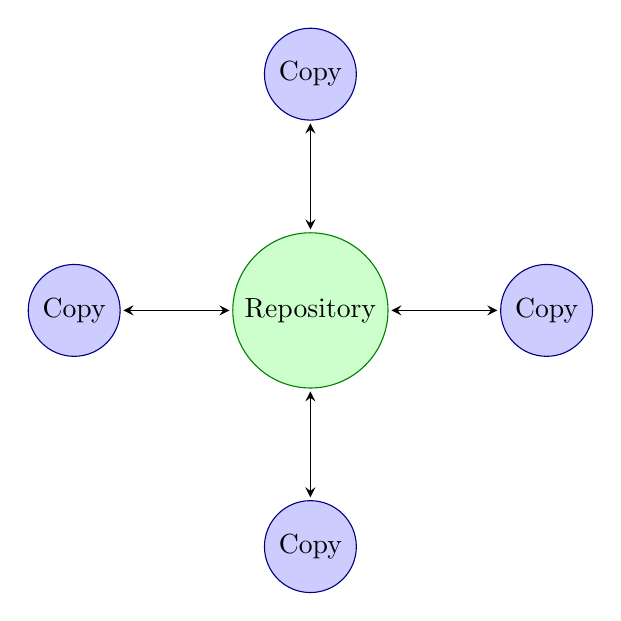
\begin{tikzpicture}
[repo/.style={circle,
		fill=green!20!white,
		draw=green!50!black,
		minimum size=10mm},
workingcopy/.style={circle,
		fill=blue!20!white,
		draw=blue!50!black,
		minimum size=5mm},
link/.style={<->, shorten <=1pt, shorten >=1pt, >=stealth, semithick}]

% central repo
\node at (0, 0) [repo] (mainrepo) { Repository };
% working copies
\node at (3,0)  [workingcopy] (copyright)  { Copy };
\node at (-3,0) [workingcopy] (copyleft)   { Copy };
\node at (0,3)  [workingcopy] (copytop)    { Copy };
\node at (0,-3) [workingcopy] (copybottom) { Copy };
% links between repo and working copies
\draw [link] (mainrepo) -- (copyright);
\draw [link] (mainrepo) -- (copyleft);
\draw [link] (mainrepo) -- (copytop);
\draw [link] (mainrepo) -- (copybottom);
\end{tikzpicture}
